\documentclass[a4paper,12pt]{article}
\usepackage[T1]{fontenc}
\usepackage[portuguese]{babel}
\usepackage{amsmath}
\usepackage{graphicx}

% Default fixed font does not support bold face
\DeclareFixedFont{\ttb}{T1}{txtt}{bx}{n}{12} % for bold
\DeclareFixedFont{\ttm}{T1}{txtt}{m}{n}{12}  % for normal

% Custom colors
\usepackage{color}
\definecolor{deepblue}{rgb}{0,0,0.5}
\definecolor{deepred}{rgb}{0.6,0,0}
\definecolor{deepgreen}{rgb}{0,0.5,0}

\usepackage{listings}

% Python style for highlighting
\newcommand\pythonstyle{\lstset{
		language=Python,
		basicstyle=\ttm,
		morekeywords={self},              % Add keywords here
		keywordstyle=\ttb\color{deepblue},
		emph={MyClass,__init__},          % Custom highlighting
		emphstyle=\ttb\color{deepred},    % Custom highlighting style
		stringstyle=\color{deepgreen},
		frame=tb,                         % Any extra options here
		showstringspaces=false
}}


% Python environment
\lstnewenvironment{python}[1][]
{
	\pythonstyle
	\lstset{#1}
}
{}

% Python for external files
\newcommand\pythonexternal[2][]{{
		\pythonstyle
		\lstinputlisting[#1]{#2}}}

% Python for inline
\newcommand\pythoninline[1]{{\pythonstyle\lstinline!#1!}}

\begin{document}
	
	\section{Equacionando o problema}

		Sendo $h_{0} = 0$ e $v_{0} = 0$

		\begin{align*}
			h &= h_{0} + v_{0}t + \frac{1}{2}gt^2 \\
			h - h_{0} &= v_{0}t + \frac{1}{2}gt^2 \\
			h &= \frac{1}{2}gt^2 \\
			2h &= gt^2 \\
			t &= \sqrt{\frac{2h}{g}}
		\end{align*}
	
	\section{Código em Python}
	
	\pythonexternal{exercicio2.py}

	
	\begin{figure}
		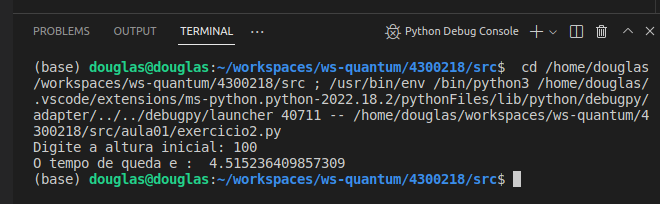
\includegraphics[width=15cm] {exercicio2.png}
		\caption{Resultado da execucao do programa}
	\end{figure}
	
\end{document}